\begin{figure}[hb]
    \centering
    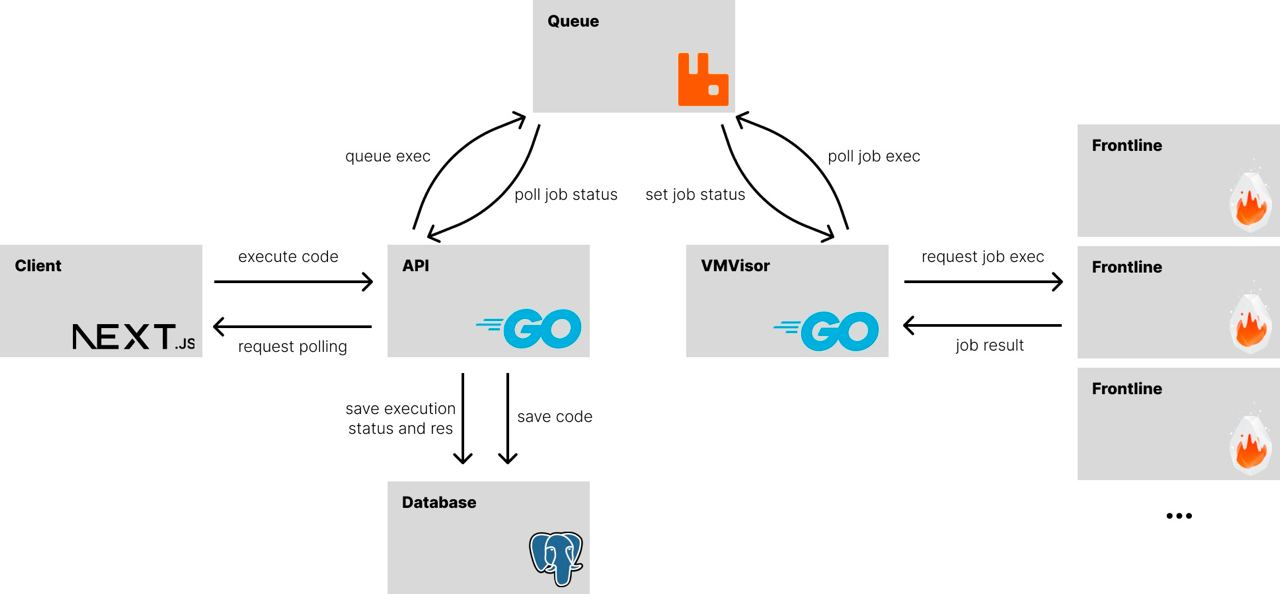
\includegraphics[width=1\textwidth]{./3-Design/design.jpg}
    \caption{معماری پروژه}
    \label{fig:architecture}
\end{figure}

\begin{table}[hb]
    \centering
    \caption{لیست سرویس ها}
    \label{table:services}
    \begin{tabular}{|c|c|}
        \hline
        سرویس ها  & توضیحات                                                                 \\
        \hline

        API       & سرویس REST API می‌باشد که وظیفه صحبت با دیتابیس و پاسخ به کلاینت را دارد \\
        \hline

        VMVisor   & مدیریت VM های ساخته و دریافت و تغییر وضعیت درخواست های اجرا روی صف      \\
        \hline

        Frontline & درون هر VM در حال اجراست و توسط پروسه فرزند کامپایلر زبان را صدا می‌زند  \\
        \hline


        Client    & کلاینت وطیفه نمایش رابط کاربری و ادیتور را دارد                         \\
        \hline
    \end{tabular}
\end{table}